\subsection{Types of data}
Now that we know that we have some kind of data as our input, we need to take a look at what this data can look like. Generally speaking, there are two types:
\begin{itemize}
  \item \sidenote{Structured data}Structured data \begin{note}like age, time, gender, class, etc.\end{note}, and
  \item \sidenote{Unstructured data}Unstructured data \begin{note}like text, audio, video, etc.\end{note}
\end{itemize}

For \textbf{structured data} we have a further subdivision into structured data types. The data types depicted in \ref{fig:1_structured_data} will be described in detail.

\begin{figure}[h]
  \centering
  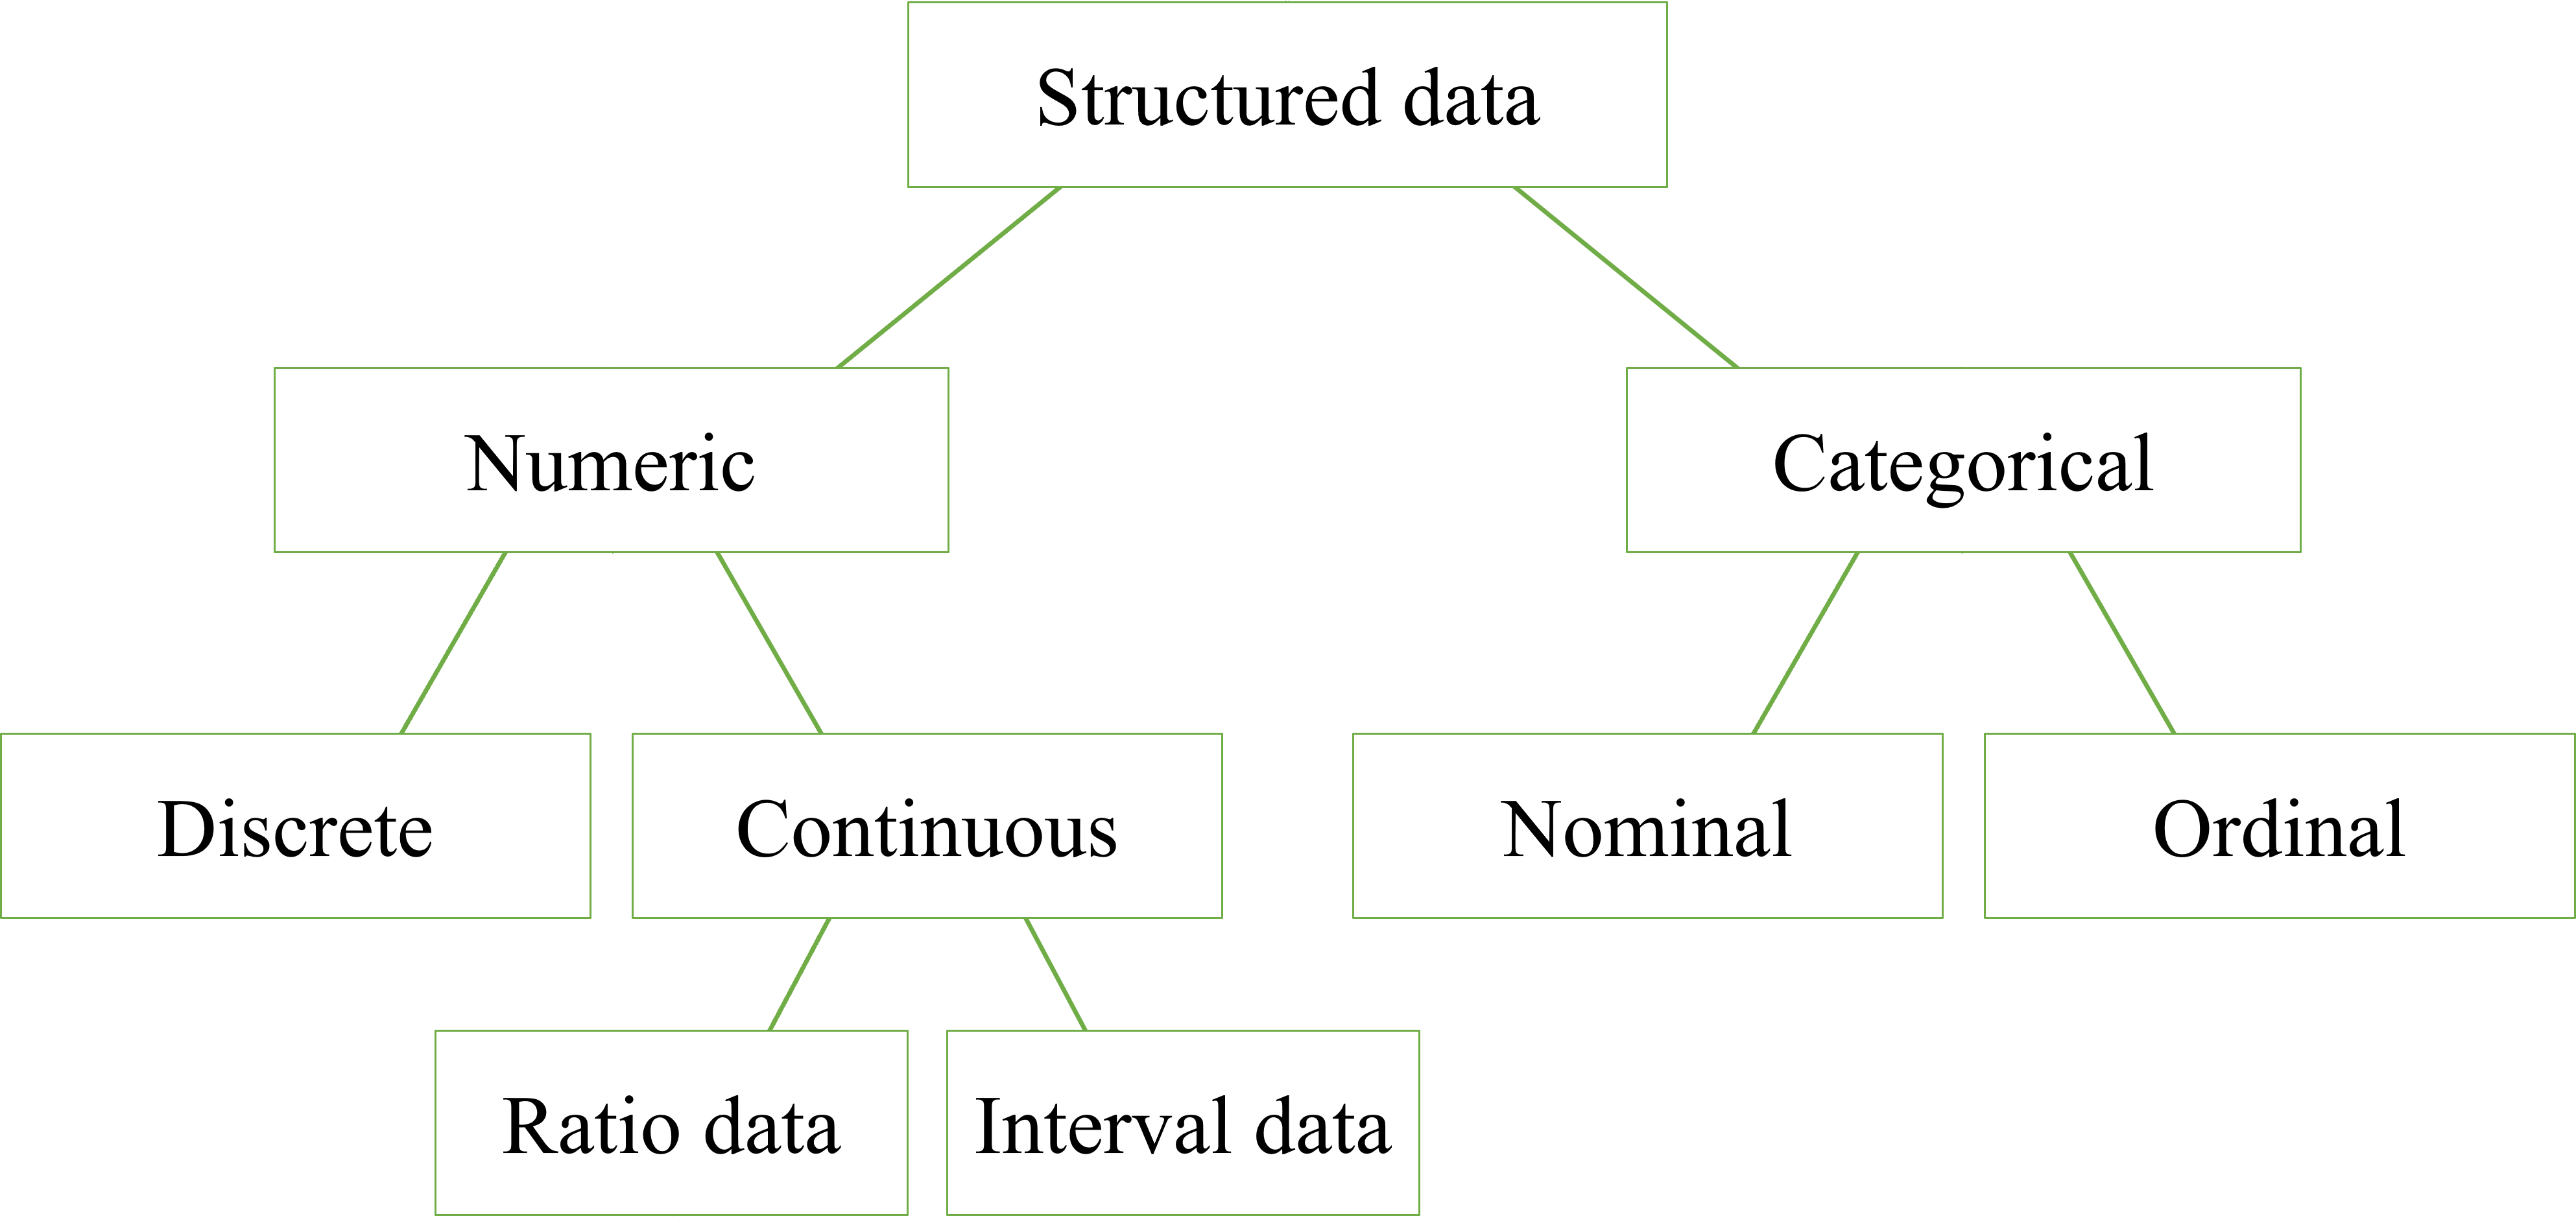
\includegraphics[width=0.9\textwidth]{assets/basics/structured_data.png}
  \caption{Overview structured data types}
  \label{fig:1_structured_data}
\end{figure}

\begin{itemize}
  \item \sidenote{Categorical data}\textbf{Categorical} data can be stored and identified based on names or labels given to them and is also known as "qualitative" data. Matching can be applied, where data is grouped based on similarities.
  
  \item Concretely, \sidenote{Nominal data}\textbf{nominal} data or naming data has a label and its characteristic similar to a noun and doesn't imply an order.
  
  \item \sidenote{Ordinal data}\textbf{Ordinal} data on the other hand is ranked, ordered, or used on a rating scale. This means, you can count and order ordinal data but are not able to measure it.
  
  \item In contrast to categorical data, we also have \sidenote{Numerical data}\textbf{numerical} data referring to data in the form of numbers instead of another language or descriptive form. It is also known as "quantitative" data. Important is the ability to be statistically and arithmetically calculated (allowing for $+, -, >, =, \dots$).
  
  \item One subtype of numerical data is \sidenote{Discrete data}\textbf{discrete} data representing countable items, that are collected in a list (finite or infinite).
  
  \item Then, there's also \sidenote{Continuous data}\textbf{continuous} data in the form of intervals or ranges. The data represents measurements with their intervals falling on a number line (so counting isn't involved).
  
  \item Continuous data can now be further distinguished. One subtype is \sidenote{Interval data}\textbf{interval} data where the data can be measured only along a scale at equal distances from each other, so only addition and subtraction operations are allowed. There is no true zero (and hence no $\cdot, /$).
  
  \item And finally, we have \sidenote{Ratio data}\textbf{ratio} data describing measurement with a defined (true) zero point.
\end{itemize}

For \textbf{unstructured data}, we just take the raw data and interpret it as a stream of bits. This goes for text, audio, images, signals, and videos exactly the same. Examples can be seen in \ref{fig:1_unstructured_data}.

\begin{figure}[H]
  \centering
  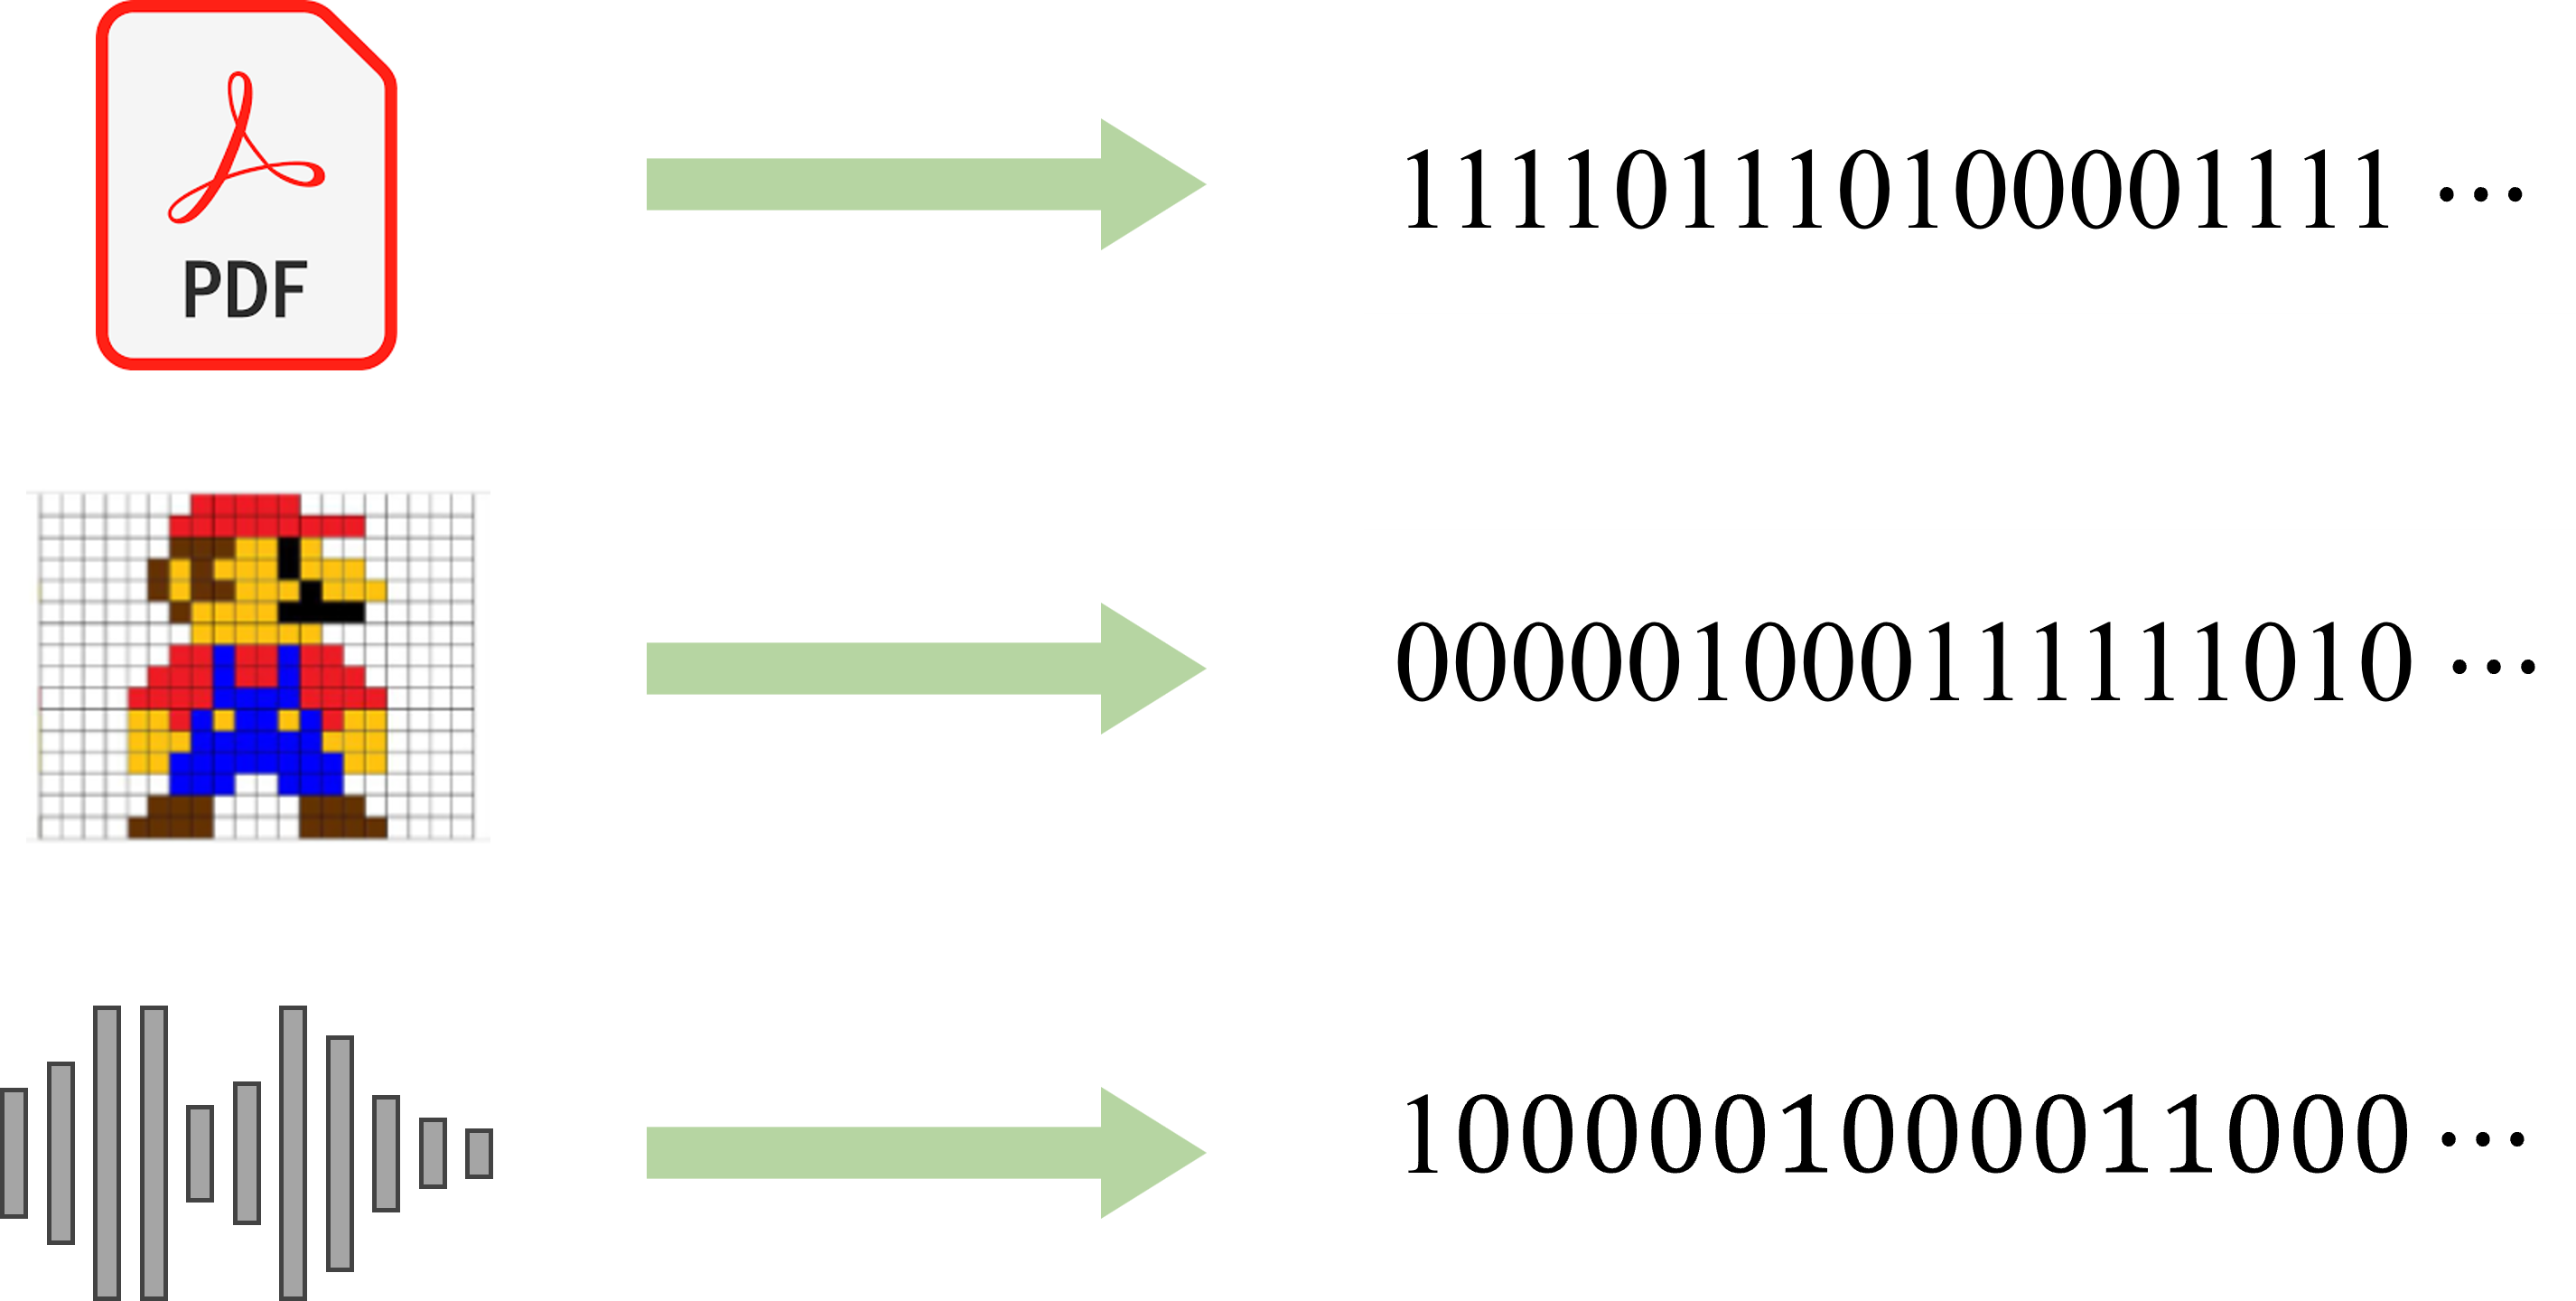
\includegraphics[width=0.4\textwidth]{assets/basics/unstructured_data.png}
  \caption{Input for unstructured data}
  \label{fig:1_unstructured_data}
\end{figure}

Data can now be stored and ordered together by putting it into \sidenote{Tabular data}\textbf{tables}. Concretely, columns represent different features (can be different kinds of data types) whereas rows describe data instances (also known as individuals, entities, cases, objects, or records). Examples can be seen in \ref{fig:1_table_data}.

\begin{figure}[H]
  \centering
  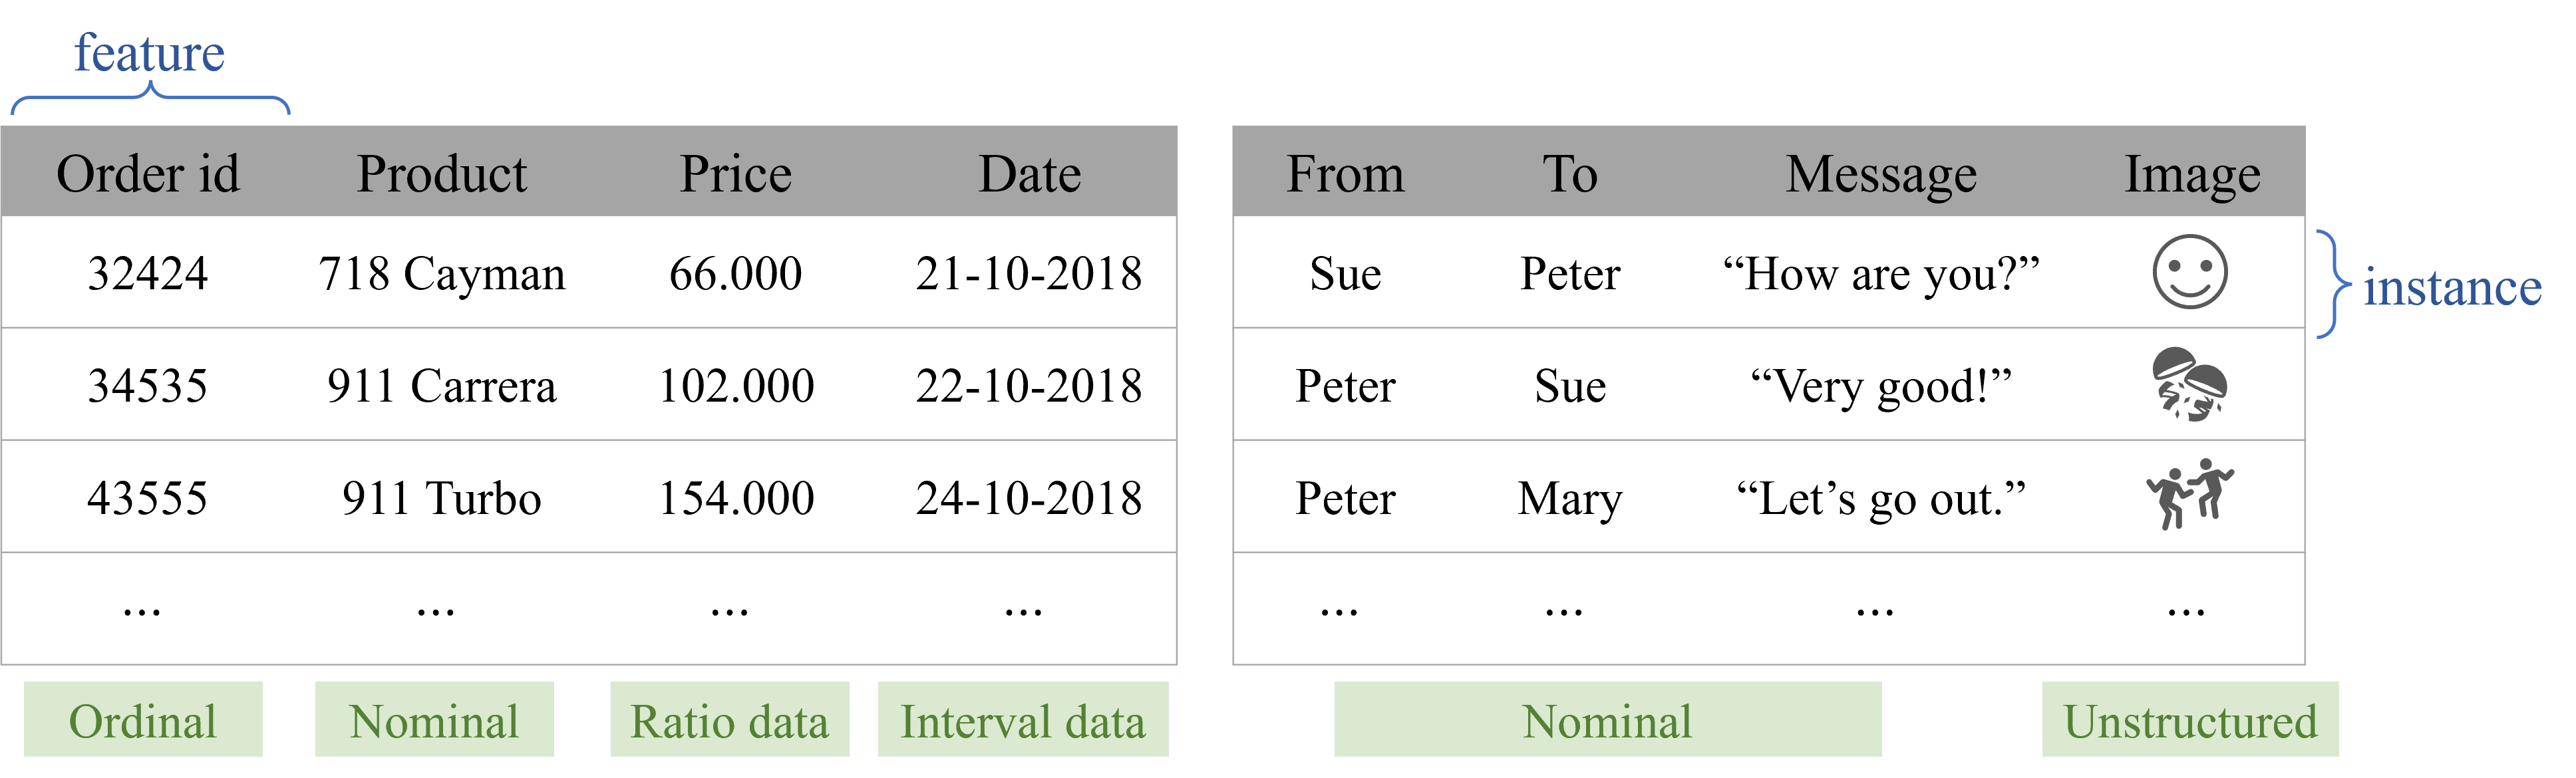
\includegraphics[width=\textwidth]{assets/basics/table_data.png}
  \caption{Table data with data types}
  \label{fig:1_table_data}
\end{figure}

Features \sidenote{Features} can now be raw or derived \begin{note}(e.g. max, min, average, rank, bin, $\dots$)\end{note}. An important aspect is time, as it cannot decrease and we usually want to predict the future based on the past. 

An important distinction to be made when it comes to tabular data is whether the items are labeled or not.
\begin{itemize}
  \item \sidenote{Labelled data}In case of labelled data we have \textbf{descriptive features} and a \textbf{target feature}.
  \begin{itemize}
    \item The \sidenote{Descriptive features}descriptive features are also known as predictor variables or independent variables.
    \item Alternative names for \sidenote{Target feature}target features are response variable, dependent variable, or also label.
  \end{itemize}
  \item \sidenote{Unlabelled data}Unlabelled data on the other hand doesn't have a selected target feature.
\end{itemize}